\makeatletter
\def\thickhrulefill
{
	\leavevmode \leaders \hrule height 1pt\hfill \kern \z@
}

\renewcommand{\maketitle}
{
	\begin{titlepage}
		\vspace*{-25mm}
		
		\setlength\fboxrule{0pt}	% suppression bordure
		\fbox
		{
			\hspace{-10mm}
			\begin{minipage}{60mm}
				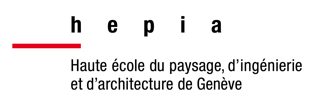
\includegraphics[width=60mm]{img/hepia-logo-300.jpg}
			\end{minipage}
		}
		\vspace{10mm}
	
	
		\begin{center}
		%\LARGE{\school}\\
		%\LARGE{\textsc{\faculty}} \\
		\smallskip\smallskip
		\large \diploma \\
		\large \subject \\
		\end{center}
	
    	\let\footnotesize\small
    	\let\footnoterule\relax
    	\parindent \z@
    	\reset@font
    	\null\vfil
    
    	\begin{flushleft}
	    	\LARGE \textbf{\@title}
    	\end{flushleft}
    
    	\par
    	\hrule height 4pt
    	\par
    	
    	\begin{flushright}
      		\large \textsc{\version} \par
    	\end{flushright}
    	
    	\begin{figure}[ht!]
    	   \centering
    	   
\includegraphics[width=100mm]{img/no_image.png}\\
    	   \textit{}
    	\end{figure}
    	
    	\vskip 20\p@
    	\vfil\null
    	
    	\begin{center}
    	Enseignant : Firstname \textsc{Lastname} \\
    	Auteur: \@author \\[1em]
    	Genève, le \today	
    	\end{center}
    	
	\end{titlepage}
  	\setcounter{footnote}{0}
}


\makeatother
\author{\authorname}
\title{\titlename}
\date{\today}
